\documentclass[../MATLAB_Primer.tex]{subfiles}
\begin{document}
The Symbolic Math Toolbox in MATLAB is a powerful tool for working with mathematical expressions analytically.  Working with symbolic functions allows you to perform a number of operations such as transforms, differentiation, and integrals without ever needing to evaluate the function numerically. It essentially emulates the pen-and-paper formulation of the mathematics. 

\subsection{Symbolic Variables}
\subsubsection{Declaration}
Symbolic variables can be declared using either the \texttt{sym} or \texttt{syms} functions. There are minor differences in the syntax between the two, and their definitions with links to the official documentation can be found below.  Generally you will wish to use \texttt{syms} when creating symbolic variables. 

\begin{table}[H]
\caption{Functions for Symbolic Variable Declaration}
    \begin{center}
        \begin{tabular}{| C{3cm} | m{12cm}|}
            \hline
            \textbf{MATLAB Syntax} & \textbf{Description}\\
            
            \hline
            \href{https://www.mathworks.com/help/symbolic/sym.html}{\color{blue}sym} & Creates symbolic variables and numbers\\
            \hline
            
            \href{https://www.mathworks.com/help/symbolic/syms.html}{\color{blue}syms} & Shortcut for \texttt{sym}\\
            \hline
        \end{tabular}
        \label{tab:symbolic_variables}
    \end{center}
\end{table}

Example 1:\\

\textit{input:}
\begin{lstlisting}
% can create symbols for exact numbers or variables
x = sym('x');   
y = sym(1/3);  

% the following output is exactly 4/3 instead of 1.3333
y+1
\end{lstlisting}
\textit{output:}
\begin{center}
    ans = 4/3
\end{center}

Example 2:\\

\textit{input:}
\begin{lstlisting}
% syms allows you to declare multiple symbols at once
syms x y z w;
\end{lstlisting}
\textit{output:}

\subsubsection{Symbolic to Numeric Conversion}
Although symbolic variables can preserve the precision of exact numbers, there are often cases where we wish to recover the numeric approximation for use in computation. This is accomplished mainly through the use of the \texttt{double} function.  The example below illustrates this symbolic-double conversion.\\

\begin{table}[H]
\caption{Functions for Symbolic to Numeric Conversion}
    \begin{center}
        \begin{tabular}{| C{3cm} | m{12cm}|}
            \hline
            \textbf{MATLAB Syntax} & \textbf{Description}\\
            
            \hline
            \href{https://www.mathworks.com/help/symbolic/double.html}{\color{blue}double(s)} & Converts symbolic variable $s$ to a numeric type with \texttt{double} precision\\
            \hline

        \end{tabular}
        \label{tab:symnum_conversion}
    \end{center}
\end{table}

Example 1:\\

\textit{input:}
\begin{lstlisting}
exact = sym(1/3);
numeric = double(exact);

disp(exact)     % display the symbolic variable 
disp(numeric)   % display numeric conversion
\end{lstlisting}
\textit{output:}
\begin{center}
    exact = 1/3,\quad numeric = 0.3333
\end{center}


\subsection{Symbolic Functions}
\subsubsection{Declaration}
Symbolic functions are built off of symbolic variables and are advantageous from an analytical standpoint. Symbolic functions can be declared similarly to symbolic variables \textbf{or} through the use of the \texttt{symfun} command. 

\begin{table}[H]
\caption{Functions for Symbolic Function Declaration}
    \begin{center}
        \begin{tabular}{| C{3cm} | m{12cm}|}
            \hline
            \textbf{MATLAB Syntax} & \textbf{Description}\\
            
            \hline
            \href{https://www.mathworks.com/help/symbolic/symfun.html}{\color{blue}symfun} & Creates symbolic functions\\
            \hline
        \end{tabular}
        \label{tab:symbolic_functions}
    \end{center}
\end{table}

There are many ways to declare a symbolic function.  The examples here provided run through several alternative methods.\\

Example 1:\\

\textit{input:}
\begin{lstlisting}
% define f(x) = 5*x^2 + (1/2)*sin(x)^2 symbolically 
syms f(x);

f(x) = 5*x^2 + (1/2)*sin(x)^2; 

formula(f)  % returns the expression associated with f
\end{lstlisting}
\textit{output:}
\begin{center}
    ans = sin(x)\^{}2/2 + 5*x\^{}2 
\end{center}

Example 2:\\

\textit{input:}
\begin{lstlisting}
% define f(x,y) = x^2 + y^2 symbolically 
syms x y;

f(x,y) = x^2 + y^2; 

formula(f)
\end{lstlisting}
\textit{output:}
\begin{center}
    ans = x\^{}2 + y\^{}2 
\end{center}

Example 3:\\

\textit{input:}
\begin{lstlisting}
% define f(x,y) = (1/3)*e^(x^2+y^2) symbolically 
x = sym('x');
y = sym('y');

f(x,y) = (1/3)*exp(x^2+y^2); 

formula(f)
\end{lstlisting}
\textit{output:}
\begin{center}
    ans = (1/3)*exp(x\^{}2+y\^{}2) 
\end{center}

Example 4:\\

\textit{input:}
\begin{lstlisting}
% define f(x,y) = x + y symbolically 
syms x y;

f = symfun(x+y,[x y]); 

formula(f)
\end{lstlisting}
\textit{output:}
\begin{center}
    ans = x + y
\end{center}


\subsubsection{Evaluating Symbolic Functions}
Symbolic functions can be differentiated or integrated without the need of numerical methods.  Additionally you can easily evaluate symbolic functions at specific points or over a domain with a numeric return type.  Some relevant functions for working with symbolic functions are included in the table below.

\begin{table}[H]
\caption{Functions for Evaluating Symbolic Functions}
    \begin{center}
        \begin{tabular}{| C{3cm} | m{12cm}|}
            \hline
            \textbf{MATLAB Syntax} & \textbf{Description}\\
            
            \hline
            \href{https://www.mathworks.com/help/symbolic/diff.html}{\color{blue}diff(f, $\sigma$)} & Returns the derivative of a symbolic function, $f$, w.r.t. parameter $\sigma$ as another symbolic function   \\
            
            \hline
            \href{https://www.mathworks.com/help/symbolic/sym.int.html}{\color{blue}int(f, $\sigma$)} & Returns the definite or indefinite integral of a symbolic function, $f$, w.r.t. parameter $\sigma$  \\

            \hline
            \href{https://www.mathworks.com/help/symbolic/subs.html}{\color{blue}subs(f, old, new)} & Substitutes parameter $old$ with parameter $new$ in a symbolic expression $f$  \\
            \hline
            
        \end{tabular}
        \label{tab:symbolic_evaluation}
    \end{center}
\end{table}

Example 1:\\

\textit{input:}
\begin{lstlisting}
syms f(x);

f(x) = x^2;

% evaluate at a point;
f(2)

% evaluate over a domain
domain = linspace(-10,10);
range = f(domain);
plot(domain, range)
\end{lstlisting}
\textit{output:}
\begin{center}
    ans = 4
\end{center}
\begin{figure}[H]
    \centering
    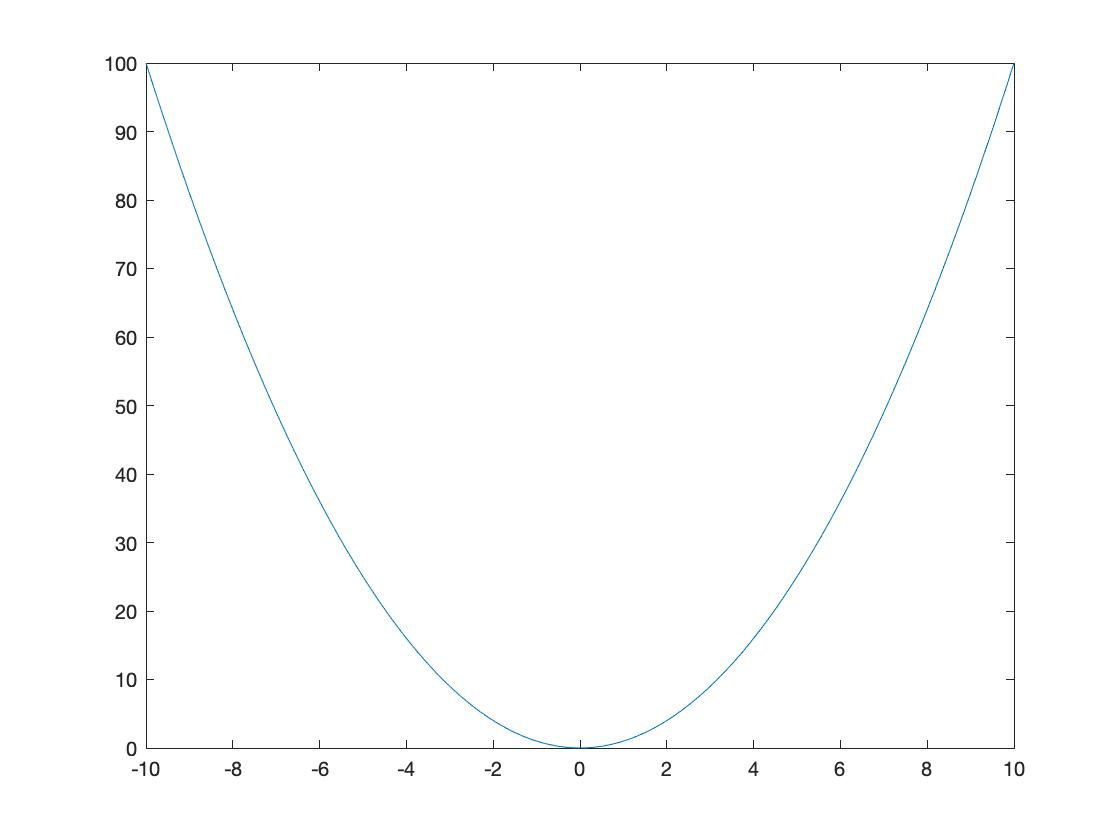
\includegraphics[width=350pt]{images/sym_parabola.jpg}
    \caption{Evaluating symbolic function over a domain}
    \label{fig:sym_plot}
\end{figure}

Example 2:\\

\textit{input:}
\begin{lstlisting}
syms f(x);

f(x) = x^2;

% can use subs to change the variable x->s 
syms s;
subs(f, x, s);
formula(f)

% can use subs to evaluate at the point s=2
subs(f, s, 2)

\end{lstlisting}
\textit{output:}
\begin{center}
    ans = s\^{}2,\quad ans(x) = 4
\end{center}


Example 3:\\

\textit{input:}
\begin{lstlisting}
syms f(x);

f(x) = sin(x^2);
df = diff(f,x)  % differentiate f(x) w.r.t x

formula(df)

\end{lstlisting}
\textit{output:}
\begin{center}
    ans = 2*x*cos(x\^{}2)
\end{center}


Example 4:\\

\textit{input:}
\begin{lstlisting}
syms f(x);

f(x) = 1/x;

% indefinite integral
indef = int(f,x);   % symbolic 
formula(indef)

% definite integral from 1 to 10
def = int(f,x,1,10)
double(def)         % numeric 

\end{lstlisting}
\textit{output:}
\begin{center}
    indef = log(x),\quad ans = 2.3026
\end{center}

\end{document}